\documentclass{standalone}

\usepackage{enumitem}
\setlistdepth{20}
\renewlist{description}{description}{20}

\begin{document}
	Both the design and implementation processes occurred simultaneously, that is the implementation of our application evolved alongside the development of its final design. During the design chapter (see \fullref{chap:design}), we only discussed the final state of the system. This was done to avoid creating any confusion with regards to what was actually created. However, throughout this chapter we will be discussing some of the mistakes made, difficulties faced, and the solutions allowing us to overcome them.

	\section{Source Overview}
		Great effort has been invested into ensuring that our implemented source-code is of a high-quality. Among other aspects, this entails conscious attention to certain factors, such as maintainability and reusability. This is especially important due to the multifaceted nature of the project.

		In particular, certain software development principles have been utilised, such as high-cohesion and low-coupling. This results with an implementation that is both easier to understand, and whose components can be easily integrated into future projects.

		Throughout the remainder of this section, we shall provide the reader with an overview of our application's source-code. This is to help establish an understanding of what exactly has been developed, and how the implementation is structured. However, for an in-depth description regarding specific detail of our code, we advise the reader to further their understanding by consulting said source-code directly. In order to ease this, high amounts of documentation have been embedded throughout the codebase.\footnote{We've omitted all unit-tests to try and keep this list concise.} \footnote{In order to retain focus on our project's primary aspects, we avoid delving too far into React Universally (see \fullref{sec:boilerplate}).}

		\begin{formal}
			\begin{description}
				\item[./]: the root directory of our project.
				\begin{description}
		        	\item[./.babelrc]: configuration file for Babel (see \fullref{sec:coreTechnologies}).

		        	\item[./.editorconfig]: configuration file for EditorConfig, providing a means for developers' to define and maintain consistent coding styles between different editors and IDEs.

		        	\item[./.env\_example]: example configuration file describing environment variables intended for use during deployment. This is provided by React Universally.

		        	\item[./.eslintignore]: configuration file containing patterns identifying specific files that we intentionally do not wish to lint. This includes third-party and post-build source-code.

		        	\item[./.eslintrc]: configuration file for our JavaScript linter (see \fullref{sec:softwareDevelopmentProcess}).

		        	\item[./.modernizrrc]: configuration file for Modernizr. This allows us to detect the supported technologies within a client's web-browser. This is provided by React Universally.

		        	\item[./.nvmrc]: configuration file stating this application's intended version of Node.js.

		        	\item[./LICENSE]: copy of the application's licence, that being \emph{GNU GENERAL PUBLIC LICENSE Version 3}.

		        	\item[./package.json]: configuration file for Node.js containing much meta-data regarding our application, such as dependencies and scripts. Extended from what is provided by React Universally.

		        	\item[./README.md]: short piece of text introducing developers to the application.

		        	\item[./TODO.todo]: todo-list containing a log of tasks completed throughout development (see \fullref{sec:softwareDevelopmentProcess}). This became somewhat disregarded towards the later stages.

		        	\item[./yarn.lock]: log of the exact dependency versions, for predictable portability. This is provided by React Universally.
		      	\end{description}

	        \item[build/]: output directory containing our source-code once it has been transpiled and passed through a module bundler. We refrain from discussing its contents in further detail.

	      	\item[client/]: directory containing browser specific source that serves no purpose server-side, not even for server-side rendering.
	        \begin{description}
	        	\item[index.js]: kickstarts our application within the client's browser. Extended from what is provided by React Universally.
	        	\item[registerServiceWorker.js]: installs the offline plugin, which instantiates our service worker and app cache to support pre-caching of assets and offline support. This is provided by React Universally.

		        \item[components/]: directory containing the React components not intended for server-side rendering.
		      	\begin{description}
	        		\item[ReactHotLoader.js]: enables React hot-loading for development builds of our application. This is provided by React Universally.
        		\end{description}

		        \item[game/]: directory containing all the Tron game functionality that is strictly only required client-side.
		      	\begin{description}
		        	\item[draw.js]: draw functionality that attaches to the canvas element of our document, enabling it to draw the graphics for our game of Tron.
		        	\item[drawdebug.js]: optional draw functionality that overlays the standard Tron graphics to provide the user with a visualisation that is more useful for debugging. In particular, highlighting the bounds for each node within our collision data-structure.
		        	\item[gameloop.js]: a version of the game loop optimised for the web-browser (for more information, see \fullref{sec:gameloopChallenges}).

		        	\item[polyfills/]: directory containing polyfills that offer workarounds for clients whose browsers lack certain functionality. This is provided by React Universally.
		      		\begin{description}
		        		\item[polyfills/index.js]: example polyfill for clients that lack the picture element.
	        		\end{description}

		        	\item[state/]: directory containing Redux functionality that powers the state of our application (see \fullref{sec:coreTechnologies}).
		      		\begin{description}
			        	\item[index.js]: entry point file which sets up our root Redux reducer and root Redux Saga (see \fullref{sec:reduxIntegration}).

			        	\item[input/]: directory containing Redux functionality for processing user-input.
		      			\begin{description}
				        	\item[host/]: directory containing the Redux functionality usable by the host user to configure the game lobby.
		      				\begin{description}
				        		\item[sagas.js]: Redux sagas used to execute actions on behalf of the game host for the current game lobby.
		      				\end{description}

				        	\item[keyboard/]: directory containing the functionality required for Redux to emit actions on keyboard input.
		      				\begin{description}
				        		\item[actions.js]: Redux actions for the key-down and key-up keyboard user-input events.
				        		\item[sagas.js]: Redux Saga which forks out to constantly listen for keyboard input from the user; distributing actions for the appropriate events.
		      				\end{description}

		      				\item[player/]: directory containing the Redux functionality usable by the user in order to control their player.
		      				\begin{description}
				        		\item[sagas.js]: Redux sagas used to execute actions on behalf of the user, so that they're able to control their game player.
		      				\end{description}
		      			\end{description}

			        	\item[lobby/]: directory containing Redux functionality enabling the user to communicate with their game lobby.
		      			\begin{description}
			        		\item[sagas]: Redux sagas used to send/receive messages between client, and the server holding the game lobby.
		      			\end{description}

			        	\item[sockets/]: directory containing the means allowing Redux to communicate, in a natural manner, with a server via WebSockets (see \fullref{sec:reduxIntegration}).
		      			\begin{description}
				        	\item[actions]: Redux actions used to establish and communicate using a WebSocket connection.
				        	\item[reducers]: Redux Reducer which attaches the WebSocket connection status to our Redux store's state.
				        	\item[sagas]: Redux sagas facilitating integration between WebSockets and Redux. 
		      			\end{description}
		      		\end{description}
	      		\end{description}
	      	\end{description}

	        \item[config/]: directory containing general configuration for our web-application and the build/deploy process. Extended from what is provided by React Universally.

	        \item[internal/]: directory containing most of the internals powering React Universally.

	      	\item[node\_modules/]: directory containing many of the third-party dependencies, as specified within our \texttt{package.json} file.

	      	\item[public/]: directory containing miscellaneous static files useful for hosting a web-application. This is provided by React Universally.

	      	\item[server/]: directory containing functionality specific to our Node.js server.
		        \begin{description}
		        	\item[index.js]: kickstarts the server component of our application. Extended from what is provided by React Universally.
		        	\item[sockets.js]: initiates the WebSocket functionality and hooks up our Tron game server, supplying the necessary Node.js dependencies for dependency injection.

		        	\item[game/]: directory containing all the Tron game functionality that must be specialised for a particular platform, in this case Node.js. This will interface with the remaining game files using dependency injection.
		        	\begin{description}
			        	\item[gameloop.js]: a version of the game loop optimised for the Node.js run-time environment (for more information, see \fullref{sec:gameloopChallenges}).

			        	\item[processes/]: directory containing the entry-points for our Node.js child processes (see \fullref{sec:lobbyConcurrency}).
		        		\begin{description}
				        	\item[aimove.js]: child process entry point used by a computer player in order to determine a move calculated using some artificial intelligence.
				        	\item[update.js]: child process entry point used by our game's state controller to update the game state.
				      	\end{description}
			      	\end{description}

		        	\item[middleware/]: directory containing middleware for our Node.js server. Extended from what is provided by React Universally, in order for compatibility with Redux.
		      	\end{description}

	      	\item[shared/]: directory containing the bulk of functionality developed for our application. Its contents are intended for use both on the client and server.
        		\begin{description}
		        	\item[components/]: directory containing our React components which compose the view layer.
		        	\begin{description}
		        		\item[App/]: directory containing the components specific to our application.
				      	\begin{description}
		        			\item[index.js]: base component of our application.
		        			\item[globals.css]: CSS style rules which apply to our application as a whole.

		        			\item[Error404]: directory containing components for a simple 404 page. This is provided by React Universally.

		        			\item[GameCanvas/]: directory containing the components for the canvas element which we draw Tron's graphics onto.
					      	\begin{description}
		        				\item[index.js]: the component representing our game canvas, including the functionality enabling it appropriately adjust in size.
							    \end{description}

		        			\item[Lobby/]: directory containing the components used to create a panel of information and options for when the user is connected to a lobby.
					      	\begin{description}
		        				\item[index.jsx]: base component for our game lobby panel. This component will initiate the WebSocket connection to the appropriate game lobby.

		        				\item[host/]: directory containing the components of our game lobby panel's host section, providing additional configurations to users who are the host of their current game lobby.
				      			\begin{description}
		        					\item[index.js]: base component containing the graphical controls for host operations.
						    		\end{description}
							    \end{description}

		        			\item[Welcome/]: directory containing the components used to create a welcome screen for when the user is not connected to a lobby.
					      	\begin{description}
		        				\item[index.jsx]: base component containing a brief introduction to our Application along with the ability to set the player name and join a random lobby.
						    \end{description}


					    \end{description}

					    \item[HTML/]: directory containing a generic component used as the foundation of a HTML document. This is provided by React Universally.
			    	\end{description}

				    \item[game/]: directory containing the majority of Tron's game code.
			      	\begin{description}
			      		\item[gameloop.js]: an abstract class of our game loop, intended to be extended upon by adding a platform specific timer.

			      		\item[ai/]: directory containing the functionality powering our computer players through the use of artificial intelligence (for more information, see \fullref{sec:design-ai}).
				      	\begin{description}
				      		\item[index.js]: perform some checks before initiating the simulations and returning the calculated move.
				      		\item[minimax.js]: deprecated simulation technique (for more information, see \fullref{sec:aiSimulations}).
				      		\item[montecarlo.js]: implementation of Monte Carlo tree search used to identify a strong move.
				      		\item[wintree.js]: data-structure used by our Monte Carlo tree search to keep a history of the executed simulations and their outcomes.

				      		\item[heuristics/]: directory containing the implemented heuristic evaluation functions which provide insight of the game state.
					      	\begin{description}
				      			\item[index.js]: calculate the heuristic scores for each player by using the distance map provided by the flood-fill algorithm.
				      			\item[floodfill.js]: perform our optimised flood-fill algorithm for a single player within the game arena.
					      	\end{description}
						\end{description}

					    \item[network/]: directory containing the core functionality powering the architecture enabling our game to be multiplayer (for more information, see \fullref{sec:networkCommunication}).
				      	\begin{description}
			      			\item[lobby.js]: class charged with managing an individual game lobby.
			      			\item[server.js]: class that processes client connections and arbitrates players within game lobbies.
			      			\item[snapshot.js]: utility functions to obtain and apply snapshot comparisons that are taken between two states.
			      			\item[statecontroller.js]: class which handles the authoritative game state (asynchronously) and can apply changes utilising lag compensation.

			      			\item[input/]: directory containing the various attachments to the player-server connection. These are primarily used to read messages sent from user players in order to perform some operation on the game lobby.
					      	\begin{description}
				      			\item[index.js]: attach a player to all other attachments contained within this directory.
				      			\item[host.js]: attach events to a player allowing them to perform host operations.
				      			\item[player.js]: attach events to a player allowing them to direct their player.
				      		\end{description}
			      		\end{description}

			      		\item[operations/]: directory containing a collection of handy operations that are applied to the game state.
				      	\begin{description}
			      			\item[collision.js]: operations used for the purpose of collision detection, including a function used to create the rectangle objects representing a line-segment composing player trails.
			      			\item[general.js]: general-purpose operations, including those to initialise the game state and rebuild the state cache.
			      			\item[player.js]: operations relating to the game state players, including their creation, removal, and safe repositioning.
			      		\end{description}

			      		\item[update/]: directory containing the various tasks performed during each tick of our game loop.
				      	\begin{description}
			      			\item[index.js]: entry point to our game loop tick updates. At the end, this will also check if the current game round has reached termination.
			      			\item[collision.js]: apply collision detection against our game state (see \fullref{sec:collisionDetection}). 
			      			\item[move.js]: move all alive players by the appropriate distance.
			      		\end{description}

			      		\item[utils/]: directory containing utility functionality that our game requires.
				      	\begin{description}
			      			\item[geometry.js]: contains some geometry functions used throughout our game, particularly by our collision detection.
			      			\item[spawn.js]: calculates the spawn position for a particular player within the game instance.

			      			\item[collision/]: directory containing the data-structures utilised by our collision detection.
				      		\begin{description}
				      			\item[grid.js]: implementation of a uniform grid.
				      			\item[object.js]: standard object interface used by collision data-structures.
				      			\item[quadtree.js]: implementation of a quadtree.
				    			\end{description}
			      		\end{description}
					    \end{description}

					    \item[state/]: directory containing the shared-scope Redux functionality that powers the state of our application (see \fullref{sec:coreTechnologies}).
					    	\begin{description}
			      			\item[index.js]: sets up the shared root Redux reducer and root Redux Saga (see \fullref{sec:reduxIntegration}).
			      			\item[configureStore.js]: set-up or Redux store to integrate with React Universally and its development workflow.

			      			\item[input/]: directory containing the Redux functionality enabling a by the user in order to control their player.
					    		\begin{description}
				      			\item[host/]: directory containing the Redux functionality usable by the host user to configure the game lobby.
						    		\begin{description}
				      				\item[actions.js]: actions which are emitted to the store in order for the user to perform host operations.
			    					\end{description}

				      			\item[player/]: directory containing the Redux functionality usable by the user in order to control their player.
						    		\begin{description}
				      				\item[actions.js]: actions which are emitted to the store in order for the user to perform operations regarding their player.
			    					\end{description}
			    				\end{description}

			    				\item[lobby/]: directory containing Redux functionality enabling the user to communicate with their game lobby.
					    		\begin{description}
				      			\item[actions.js]: actions relating to the user and their relationship with the game lobby.
				      			\item[reducers.js]: reducers relating to the user and their relationship with the game lobby.
			    				\end{description}
			    			\end{description}

					    \item[utils/]: utility functions provided by React Universally.
		      	\end{description}
	    \end{description}
    \end{formal}

	\section{Notable Challenges}
		\subsection{Game Loop} \label{sec:gameloopChallenges}
			Constructing the game loop is a seemingly simple task. In essence, it is a callback that some timer would make a call to at some fixed interval equal to our tick-rate. However, there were a number of quirks related to JavaScript's standard API which made this task not as straightforward as initially expected.

			On the client, we are able to use JavaScript's \emph{window.requestAnimationFrame()} \parencite{JsRequestAnimationFrame} function. This is called whenever the canvas is preparing to draw the next frame, giving us the opportunity to update the game state - basically hijacking the internal loop used within the browser. This technique worked during the early stages of development, but when we sought to run the game on the browser; it soon became apparent that obviously this function wouldn't exist in a Node.js environment. So, a separate solution needed to be realised.

			Research turned in the direction of JavaScript's standard built-in timer, \emph{setTimeout()} \parencite{JsSetTimeout}. However, after some short tests, said timer was concluded to be improper for the task as it did not tick with sufficiently reliable accuracy - often too late by many milliseconds. However, there existed an alternative function, \emph{setImmediate()} \parencite{JsSetImmediate}. 

			Sadly, this function occupied a high amount of system resources due to it ticking at an incredibly high, and uncontrollable frequency. This resulted with us having to internally disregard calls if a tick was not scheduled.

			Thankfully, after extensive research online, it was discovered that this problem has been tackled by others. A proposed solution \parencite{JsGameLoop} was suggested that recommends to use \emph{setTimeout()} as the primary timer function then, when we enter the window of potential error, switch to \emph{setImmediate()} providing us with a far greater accuracy. This seemed to work very well!

		\subsection{Head-on Player Collisions}
			Within the game loop, during the update process of single tick, we first move each and every alive player. Afterwards, we perform a series of checks to identify which players have crashed. Once all players have been checked, we process said newly crashed players by officially \emph{killing} them - which mercifully only entails switching their alive flag to \texttt{false} and reposition them to their theoretical position at the exact moment of impact.

			However, once we began testing, a bug was discovered that players would be repositioned to seemingly incorrect locations after a collision. After further investigation, it was clear that this unexpected behaviour only occurred in the case where two players would collide in a head-on collision, that is they were travelling in opposing directions and met one-another.

			After further thinking with regards to the problem, a solution was devised that modified the way in which players were repositioned. Instead, we would backtrack a player by an amount calculated by half the sum of the overshoot and overlap of the two colliding players. However, this was only necessary for the case in which a head-on collision had occurred. For more information, please see \fullref{itm:headCollision}

		\subsection{Mutability}
			Initially, the game's state was developed to be an immutable object; where all functions made no changes to the given game state, but instead returned an entirely new object with the desired changes applied. This helps to reduce obscure bugs and makes the code far easier to test - especially for unit tests.

			However, it also required performing a deep copy of the game state prior to any single change to be made. This is an extremely costly operation to be performing within a game loop, specially when it would have to be performed several times per tick. Realising this wasn't viable, the application was modified to internally use a mutable game state and to manually copy it where need be (e.g. for lag compensation, see \fullref{sec:lagCompensation}).

			Irritatingly, this caused some difficult to trace bugs. One of the most notable of these was related to copying the game state and collision data-structure within our game state's cache. In short, each object within the collision data-structure keeps a reference to the player which created it. When we then copied the game state, the stored objects did not have their player references updated to match those of the newly created player objects themselves. This resulted in faulty collision detection, related to the workings of our lag compensation. However, the bugs have since been fixed.

		\subsection{Collision Data Structures}
			In the early stages of the game's development, we would check every object within the arena when searching for collisions. Although this method worked well, and didn't result in any noticeable lag, further research into game development revealed how commonplace spatial data-structures were. This highlighted that our current collision detection mechanic was an urgent area for plausible improvement.

			Progress on the game soon advanced and the use of the hierarchical structure of a quad-tree was implemented and integrated into our game's collision detection, to help reduce the total search space when checking for collisions. This did show some considerable performance gain. However, after playing the game, it became apparent that trail line-segments were almost always intercepting multiple nodes - making the need for a hierarchical data-structure somewhat meaningless.

			Hence, a uniform grid was instead implemented and integrated to help optimised our game's collision detection. A uniform grid also has the perk of being far easier to deal-with and works well for the case of Tron.

			Also, to aid in both the creation and debugging of these two spatial data-structures, the game features a special \emph{debug} mode which would visualise the bounds for each node onto the game arena in the form of a semi-transparent overlay.

		\subsection{AI Simulations} \label{sec:aiSimulations}
			As per our design, the game's computer players were powered by an artificial intelligence that ran simulations using a variant of the minimax algorithm \parencite{minimax} that featured alpha-beta pruning \parencite{alphaBeta} to avoid looking down unnecessary branches of the game tree; improving performance.

			However, it was taking far too much time in order for the AI to calculate a suitable move. By the time the AI had calculated a move, the game state would've significantly progress; making their move now redundant - often leading to their undesired death.

			There existed two clear ways in which this performance issue could be tackled. We could either restrict the breadth of our game-tree search, or restrict the depth. Restricting the depth of our AI's game-tree search exponentially reduced its ability to make educated moves - it performed extremely poorly. On the other hand, restricting the breadth of our game-tree search was highly dependent on the situation the AI player is current in; as many of the possible early moves are never simulated.

			This inspired the idea to migrate to using the Monte Carlo tree search algorithm, as discussed in \fullref{sec:design-ai}. This allowed our AI to only explore branches of the game-tree that seemed promising; ignoring those branches that almost always led to poor outcomes.

		\subsection{AI Concurrency} \label{sec:aiConcurrency}
			In the early iterations of the game's artificial intelligence, the move for a computer controller player would prepare to calculate their next move of a tick; limiting the duration of the entire simulation process to at the most \textless 16 milliseconds. However, it soon became very apparent that this was an inadequate amount of time.

			This provoked research into the possibility of running our artificial intelligence concurrently with the rest of the game, allowing simulation to take any pre-defined amount of time. Irritatingly, as developing the artificial intelligence was the final stage of the game's development, I then discovered that Node.js is strictly a single-threaded environment. This was an absolutely devastating discovery...

			Thankfully, after an extortionate amount of research, Node's \texttt{child\_process} module \parencite{nodeChildProcess} was discovered and successfully integrated into our game sever. This was the cause for a lot of hassle, especially in regards to integration the build workflow provided by React Universally.

			In short, this Node module allows us to create a fork of an entirely new, and separate Node process capable of communicating with our main process. Not only did this allow us to execute our artificial intelligence's simulations without blocking our game loop, but it also reduced the time in which we kept our Node event loop occupied. It is critical for our Node event loop to not be used for computationally demanding tasks, as they prevent our server from processing time-sensitive requests such as processing actual user-input or even serving up the application's static files.

			Despite this, it still seemed as though our artificial intelligence was preventing our event loop from spinning fast enough. After extensive debugging, it was determined that the cause for this delay was due to the fact lag compensation was being applied after we had received the suggested move from our artificial intelligence. This greatly hindered the game's experience, as it made game-play sluggish and inaccurate; obviously this type of behaviour was unacceptable.

			This spawned a large-scale redesign regarding how the game lobby class dealt with the game state. Previously, the lobby, and therefore the main thread, would not only be responsible for running our tick updates to the state, but also for applying the sequence of updates required during lag compensation. However, the greater amount of time we have to compensate for equals a greater amount of time it takes to perform the compensation. This caused our Node event loop to get severely, and frequently held-up.

			The problem was solved thanks to the development of our \texttt{StateController} class. Each game lobby instance would, within its constructor, instantiate a new instance of this \texttt{StateController} class. Within this \texttt{StateController} instance would live a separate process that was solely dedicated to applying individual updates to the game state. For a more in-depth description, see \fullref{sec:lobbyConcurrency}.

		\subsection{AI Timing} \label{sec:aiTiming}
			Many aspects of the application rely upon the use of concurrency. Concurrency holds many benefits, particularly when it comes to performance. Irritatingly, it massively complicates aspects reliant on determinism. This became particularly evident when implementing the game's artificial intelligence. The artificial intelligence is to operate alongside concurrent tasks, such as updating the game state (see \fullref{sec:lobbyConcurrency}) and for even running the AI simulations (see \fullref{sec:aiConcurrency}).

			\begin{figure}[!htbp]
				\centering
				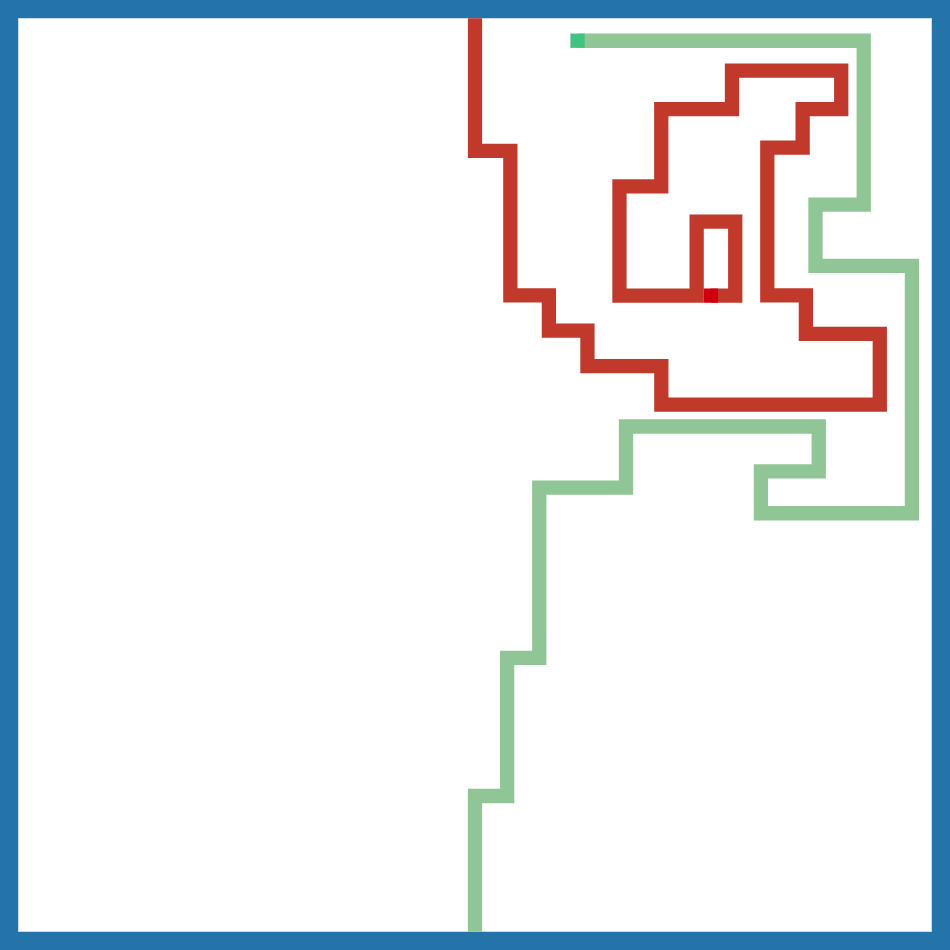
\includegraphics[width=.8\textwidth]{resources/images/aiclosecall.png}
				\caption{Diagram depicting a \enquote{close-call} situation gone wrong for an artificial intelligence controlled player (red) against a human controlled player (green).}
			\end{figure}
			\FloatBarrier

			However, our artificial intelligence was previously designed to run simulations under the assumption it had full control over the exact time in which moves could be played. The AI would spend a fixed amount of time running simulations centred around a turn-based model of our implemented game. Once all players had taken their respective turns, the game state would be updated, using a progress time equal to the minimum time required before changing move, leading to our simulations converging on strategies which could never be carried out. This is because the strategies depended on future moves being played at specific times, these times did not coincide with the fixed amount of time allocated to running the simulations. The solution to this issue was quite simple, the simulation's state update would use a time progression equal to the duration of the previous AI move calculation. This would give some indication as to when our AI would play their next move. Although not a perfect solution, manipulating the time-progression between state updates, did alleviate much of the negative impact.

		\subsection{Technology Integration}
			Some of the most prevalent issues faced were those indirectly related to the project. Specifically the issues that came about due to the discretional use of third-party libraries, and other technologies.

			\subsubsection{Redux} \label{sec:reduxIntegration}
				Redux did a pretty superb job in handling our view's state. It kept our client's view layer reflecting the current game state (see \fullref{sec:coreTechnologies}). It even played a critical role in many of the tasks occuring behind the scenes, that is those not directly related to our game's state. Despite its successful integration into our application, it was the spawn of many challenges.

				For example, Redux is not natively equipped to deal with asynchronous events; such as communicating with the server, or detecting user keyboard input. Fortunately, there exist many additional libraries which tackle this problem. One of the asynchronous libraries is Redux Saga \parencite{reduxSaga}.

				Redux Saga is a middleware that can be attached to Redux. It is used in conjunction with the new JavaScript generators, to make dealing with asynchronous code in a React/Redux application easier and more natural to work with. The use of generators play as an alternative to callbacks, which can quickly grow to become out-of-hand. In principle, it builds upon the saga pattern \parencite{sagas}.

				For most jobs, Redux Saga is quite simple to use. However, integrating Redux Saga with WebSockets proved to be quite complicated - especially with regards to the use of JavaScript generators.

				Our implemented solution begins by first immediately requesting then establishing a WebSocket connection with the server, and proceeds to maintain said connection. A saga is then set-up and tasked to constantly listen out for messages from the server, and upon receiving a message will spit out the appropriate Redux action containing the payload. A write saga is also set-up which listens for actions emitted to the store from the client. Once an action is received, it is appropriately packaged into a payload and shot off to the server using the maintained WebSocket connection. This WebSocket/Redux Saga adapter works very well, and is written in a generic manner, decoupled from the rest of the application, in order for it be feasibly integrated into other projects.

			\subsubsection{Node.js Child Process}
				Both the networking and artificial intelligence aspects of our application rely heavily on the use of Node.js's child process module. This allows us to delegate computationally expensive tasks to be computed concurrently within a separate process. However, as threading is not supported, we are unable to share memory between any two processes. As an alternative, we were able to serialise our game state and communicate that to our separate process. This was the cause of a serious issue. During development our application was experiencing some odd unexpected behaviour - input seemed sluggish at times. After some rigorous benchmarking, it was discovered that the time required to serialise, and communicate our game state to a separate process was dangerously greater than the time spent on the task inside the process. In fact, it would often take longer than several ticks to apply a single update to the game state.

				After extensive debugging, a pattern emerged in that as the elapsed time of a single game of Tron grew, the communication delay when messaging our separate process also grew. After some more analysis, communicating the game state's cache was identified as being the primary cause of this extra delay. This was due to the serialised representation of our cache occupied too much memory. Although not a perfect solution, our application now disregards game state cache when communicating with a separate process. On the receiving side of communication, the cache is efficiently rebuilt using data from the remainder of the game state. This solution produced wonderful results.
\end{document}